\documentclass[runningheads]{llncs}

\usepackage[T1]{fontenc}
\usepackage{graphicx}
\usepackage{amsmath}
\usepackage{amssymb}
\usepackage{booktabs}
\usepackage{array}
\usepackage{microtype}
\usepackage[hidelinks]{hyperref}
\renewcommand\UrlFont{\rmfamily}

\newcommand{\pass}{\checkmark}
\newcommand{\fail}{$\times$}
\graphicspath{{figures/}}

\begin{document}

\title{ProtoHedge in Real Option Markets: Near-Parity with Deep Hedging and Explanations that Link New Crises to Past Ones}
\titlerunning{ProtoHedge in Real Option Markets}

\author{Yanis Zaim\inst{1} \and Sayak Chakrabarty\inst{2} \and Imon Banerjee\inst{2}}
\authorrunning{Y. Zaim et al.}
\institute{Columbia University, New York, NY, USA\\
\email{ymz2108@columbia.edu} \and
Northwestern University, Evanston, IL, USA\\
\email{\{sayak.chakrabarty,imon.banerjee\}@northwestern.edu}}

\maketitle

\begin{abstract}
ProtoHedge makes a learned hedging policy interpretable by writing each decision as a weighted average of
actions attached to real past market states, its prototypes. In simulated markets it stayed within half a
percent of Deep Hedging. We ask whether this carries over to real option markets, and whether its
explanations are faithful there. On twenty years of US option data for ten underlyings, we hedge European
and Asian calls with the same inputs, tuning budget and checkpoint rule for both methods, and evaluate once,
on 2022--2024, with pre-declared contrasts. On the original paper's metric ProtoHedge is never detectably
behind Deep Hedging, but both methods hedge only once they are set up to do so; with the original settings
neither does. The price of interpretability is a wider hedging error: ProtoHedge removes 89\% and 85\% of
the unhedged risk, against 93\% and 89\% for Deep Hedging. A pre-declared audit shows that its explanations
are stable, name the prototypes that drive each decision, and draw on past crises when markets are
stressed. Whether they reflect visible similarity depends on the layer: with the released encoder the named
prototype is usually not the most similar past state, with the authors' simpler plain-distance layer it
usually is. During the March 2020 crash, plain-distance models trained on 2005--2018 explained their hedges mainly by
days of the 2008--09 financial crisis.

\keywords{Interpretable machine learning \and Prototype networks \and Explanation faithfulness \and Deep hedging \and Option markets}
\end{abstract}

% ------------------------------------------------------------------------------------------------
\section{Introduction}

Hedging a derivative means trading other instruments so that the combined position loses as little as
possible, whatever the market does. Deep Hedging (DH) \cite{buehler2019deep} learns such trading policies
from data with a neural network, with transaction costs, position limits and the hedger's risk preferences
built into the training objective. Its decisions come from a black box, however: a risk manager cannot see
why a particular hedge was put on, which matters when decisions must be justified and when a model meets
market conditions unlike those it was trained on \cite{rudin2019stop}.

ProtoHedge (PH) \cite{faloughi2025protohedge} makes the decision its own explanation. It replaces the
network's output layer with a prototype layer: every hedge is a weighted average of actions attached to a
small set of real states visited during training, the prototypes, and the weights measure how similar the
current state is to each of them. In simulated Black--Scholes and stochastic-volatility markets PH stayed
within half a percent of DH on the authors' utility, and the authors suggested that a decision could be
explained by its similarity to a recognisable past situation, such as ``a 2008-style financial crisis''.

Both claims were made in simulation, where data are plentiful, training and test markets are identical, and
a prototype is a simulated state with no history. Real option markets differ on all three counts. One
underlying offers about a hundred non-overlapping months of training data; the test years differ from the
training years; and a prototype is an actual trading day whose meaning a reader can check. We therefore ask
two questions. (Q1) Does PH stay close to DH on real option data, in a comparison that is fair to both?
(Q2) Are its explanations faithful to the model and meaningful in market terms? Our contributions are:

\begin{itemize}
\item \emph{A controlled test on twenty years of US option data}: ten underlyings, European and Asian
calls, identical inputs, tuning budget and checkpoint rule for both methods, and one pre-declared
evaluation on 2022--2024. On the original metric PH is never detectably behind DH, as in simulation. With
the original settings neither method hedges on real data; we identify why and how to fix it. The cost of interpretability is a wider hedging error than DH's, larger than in simulation and
shrinking with more training data.
\item \emph{A pre-declared audit of prototype explanations on market data.} The explanations are stable and
name the prototypes that drive each decision; prototypes over-represent historical crises and gain weight
when markets are stressed. During the March 2020 crash, plain-distance models trained on 2005--2018
explained their hedges mainly by days of the 2008--09 crisis. With the released encoder layer, however, the
named prototype is usually not the most similar past state, because training moves the encoder's notion of
similarity away from the visible market features. The authors' earlier plain-distance layer passes this test, and we recommend it
whenever explanations are to be checked.
\end{itemize}

% ------------------------------------------------------------------------------------------------
\section{Background and Related Work}

\paragraph{Learned hedging.} Let $x_t$ be the state observed at decision $t$ and $h_t$ the positions held
afterwards. DH parameterises the decision with a feed-forward network $\pi_\theta(x_t)$ and trains $\theta$
by gradient descent through many price paths, maximising a risk-adjusted utility of the terminal outcome,
typically an optimised certainty equivalent such as CVaR \cite{rockafellar2000,bental2007oce,buehler2019deep}.
Later work builds no-transaction bands into the network \cite{imaki2021notransaction}, removes the drift of
historical data \cite{buehler2021drift}, or treats hedging as reinforcement learning
\cite{halperin2020qlbs,kolm2019dynamic,cao2021deep,vittori2020option}. On historical option data, Ruf and
Wang found that linear regressions on standard sensitivities hedge about as well as neural networks
\cite{ruf2022hedging}, and Mikkil\"a and Kanniainen trained deep hedging policies on historical option data
\cite{mikkila2023empirical}; \cite{ruf2020review} reviews the field. We are not aware of an evaluation of an
interpretable learned hedging policy on historical option data.

\paragraph{ProtoHedge.} PH keeps DH's training objective and replaces $\pi_\theta$ by
\begin{equation}
\pi(x)=\sum_{k=1}^{K} w_k(x)\,a_k,\qquad w_k(x)=\frac{\exp(-d(x,p_k))}{\sum_{j=1}^{K}\exp(-d(x,p_j))},
\label{eq:proto}
\end{equation}
where $p_1,\dots,p_K$ are the prototypes and $a_k$ their attached outputs. The prototypes are fixed before
training: a DH agent is trained first, the states it visits on the training paths are clustered by $k$-means
\cite{macqueen1967}, and each cluster centre is replaced by the nearest visited state, so that every
prototype is a real state with a date. Only the $a_k$ and the distance $d$ are learned. Two distances appear
in the authors' work. The released code uses an encoder, $d(x,p)=\lVert f(\tilde x)-f(\tilde p)\rVert^2$,
where $f$ is a two-layer network applied to the standardised state $\tilde x$. The authors' notebooks record
an earlier \emph{plain-distance} layer, $d(x,p)=\sum_j\lambda_j(\tilde x_j-\tilde p_j)^2$ with learned
weights $\lambda_j>0$, which measures similarity directly in the standardised input features. We report
both; the released encoder is our main PH model.

\paragraph{Evaluating prototype explanations.} Prototype networks explain a decision by pointing at similar
training cases \cite{li2018prototypes,chen2019looks} and are interpretable by construction
\cite{rudin2019stop}. Their similarity is usually computed in a learned latent space, which need not agree
with similarity in the inputs a person sees \cite{hoffmann2021looks}. Explanations are therefore best judged
by functional tests rather than by examples alone \cite{doshivelez2017rigorous,nauta2023anecdotal}: whether
the evidence they name is necessary for the decision, whether they survive small changes of the input
\cite{alvarezmelis2018robustness}, and how they compare with those of an untrained model
\cite{adebayo2018sanity}. Section~\ref{sec:explain} adapts such tests to prototype hedges and adds a test of
correspondence with real market events.

% ------------------------------------------------------------------------------------------------
\section{Data and Task}
\label{sec:data}

\paragraph{Hedging task.} Each episode has $T=20$ daily decisions. At the start the hedger is short one
at-the-money synthetic call on the underlying, either European, paying $\max(S_T-S_0,0)$, or
arithmetic-average Asian, paying $\max(\bar A-S_0,0)$, where $\bar A$ is the mean of the 20 closing prices
after the start \cite{kemna1990asian}. The hedger trades the underlying and one listed call on it. With
prices $P_t\in\mathbb R^2$ divided by $S_0$, positions $h_t$ after trading at $t$, trades
$a_t=h_t-h_{t-1}$, cost $\kappa_t$ per unit traded and payment $H\le 0$, the outcome is
\begin{equation}
O=H+\sum_{t=0}^{T-1}h_t^{\top}(P_{t+1}-P_t)-\sum_{t=0}^{T-1}\kappa_t^{\top}\lvert a_t\rvert .
\label{eq:outcome}
\end{equation}
The \emph{hedging error} $E=O+V_0$ adds the model value $V_0$ of the liability at the start
(Black--Scholes \cite{black1973pricing}, or a moment-matching approximation for the Asian call, with the
listed call's implied volatility), so that a perfect hedge has $E$ close to zero on every path. Positions and
daily trades in each instrument are limited to $[-1,1]$. Costs follow the original study: $0.0002\,S_t$ per
share and $0.02\,\nu_t+0.0002\,\Delta_t+0.0005\,C_t$ per listed call, where $\nu_t$, $\Delta_t$ and $C_t$
are the call's vega, delta and mid price.

\paragraph{Data.} We combine OptionMetrics IvyDB US option quotes with CRSP prices
\cite{wrdsOptionMetrics,crspStock} for AAPL, IWM, NVDA, QQQ, SPY, TLT, XLE, XLF, XLK and XLV over
2005--2024: two stocks, broad and sector equity funds, and a Treasury bond fund. The calendar is split first:
training ends in 2018, validation covers 2019--2021 and testing 2022--2024, with a 20-day gap at each
boundary so that no episode straddles two periods. For every start date we pick, using that date's
information only, one listed call with a positive bid, a non-crossed offer, 20--40 days to expiry and a
strike within 10\% of spot (closest to the money and to 30 days, then the tightest spread), and keep that
contract for the whole episode, which avoids implicit rolls between contracts. This gives 20,537 training,
6,881 validation and 6,977 test episodes. Episodes start on consecutive trading days and overlap in 19 of
their 20 days, so the roughly 2,000 training episodes of a ticker contain only about 100 non-overlapping
months. Each day a policy observes the underlying and listed-call prices, the time left, the listed call's
implied volatility, log-moneyness and time to expiry, its own two positions and, for the Asian call, the
running average; it never sees anything after the decision time.

% ------------------------------------------------------------------------------------------------
\section{Protocol}
\label{sec:protocol}

\paragraph{Three setups.} In each setup both methods receive identical inputs, objective, output meaning
and training. (i)~\emph{The original paper's settings}: the output is a trade, the objective is CVaR at 50\%
of the outcome $O$, the state holds the two prices, the time left and the positions, DH has width 20 and PH
$K=100$ prototypes. (ii)~\emph{Equal tuning with the original objective}: the tuned configuration of (iii),
trained on CVaR$_{50}(O)$. (iii)~\emph{Trained to hedge}, the main setup: the output is a correction to the
liability's model delta, $h_t=(\Delta^{\mathrm{liab}}_t,0)+\pi(x_t)$, and the objective is the variance of
$E$. In all setups inputs are standardised with training statistics, outputs are bounded smoothly and start
near zero, and the position limits use a straight-through clamp, so that a policy cannot get stuck at a
limit.

\paragraph{Equal tuning budget.} Both methods received the same search on the validation data of three
development tickers (SPY, TLT, NVDA): three output meanings, three objectives, two state sets, and five sizes
per method (DH widths 8 to 256; $K$ from 5 to 100 for each PH layer). Mean validation rank selected $K=10$
for both PH layers and width 128 (depth 3) for DH, which tied with width 256 and was preferred as the size
closer to the original. These configurations were then frozen for all ten tickers.

\paragraph{Training.} Adam with learning rate $10^{-3}$ and batch size 32, at most 2,000 epochs, stopping
after 150 epochs without improvement; every fit keeps the epoch with the best validation objective.
Prototypes come from a width-20 DH agent trained in the same setup, as in the original recipe. The main setup
is trained with five seeds per ticker and option, the others with three. A fit with more dispersion than the
unhedged position counts as failed and stays in every average. All 1,120 fits passed an integrity check of
budget, checkpoint, reload, independent re-simulation, position limits and prototype provenance; no
main-setup fit failed.

\paragraph{Measures.} The \emph{original metric} is CVaR$_{50}(O)$, the mean of the worst half of outcomes,
reported like the original paper as the gain over not hedging (higher is better). The \emph{share of risk
removed} is $1-\mathrm{std}(E)/\mathrm{std}(E_{\mathrm{unhedged}})$. The \emph{worst-5\% loss} is
CVaR$_5(E)$, the mean of the worst 5\% of hedging errors (closer to zero is better). Results are equal-weight
averages over tickers of averages over seeds.

\paragraph{Inference.} Strategies are compared on the same episodes. Intervals come from a circular block
bootstrap \cite{politis1992} that resamples whole calendar dates in blocks of 20 days and keeps every
ticker's episode for each date, so that a market-wide shock stays in all tickers at once (2,000 draws). The
twelve pre-declared primary contrasts (PH $-$ DH, DH $-$ delta hedge and PH $-$ delta hedge, on
$\mathrm{std}(E)$ and CVaR$_5(E)$, for both options) are Holm-adjusted \cite{holm1979simple}.

\paragraph{One evaluation.} The test period was examined in an earlier version of this study with different
models. All choices in the present study were made on training and validation data and recorded before the
corresponding runs, and the test episodes were evaluated once, with a fixed specification. The explanation
tests of Section~\ref{sec:explain} were designed after that evaluation; their pass marks were recorded before
they were run, and we report them as exploratory.

\paragraph{Correctness check.} Running the authors' unmodified code reproduces their simulated result
(Table~\ref{tab:original}, top). In 2 of 5 Black--Scholes restarts, however, PH did not train (gaps of
$-23\%$ and $-30\%$); the original paper reports a single run.

\paragraph{Use of AI tools.} In line with the symposium's policy we disclose that an AI assistant (Claude,
Anthropic \cite{anthropicClaude2026}) was used to implement and run the experiment and analysis code, to
draft the pre-declared protocols, and to draft and edit this manuscript; an earlier version of the data
pipeline was written with OpenAI Codex \cite{openaiCodex2026}. The authors directed the study, reviewed the
protocols, code, results and text, and take full responsibility for the content.

% ------------------------------------------------------------------------------------------------
\section{Does ProtoHedge Match Deep Hedging on Real Data?}
\label{sec:results}

\begin{table}[t]
\caption{The original paper's comparison on simulated and real data. Gain over not hedging in CVaR at 50\%
of the outcome $O$ (fractions of the initial price; higher is better), PH minus DH with 95\% interval, the
difference relative to DH's utility, and the share of risk removed. Real data: test period 2022--2024, ten
tickers weighted equally, seeds averaged. $^{\dagger}$Interval computed after the main evaluation.}
\label{tab:original}
\centering
\scriptsize
\setlength{\tabcolsep}{2.1pt}
\begin{tabular}{@{}>{\raggedright\arraybackslash}lrrlrrr@{}}
\toprule
Setting & DH gain & PH gain & PH $-$ DH [95\% interval] & $|U_{\mathrm{DH}}|$ & Rel. & Removed \\
 & & & & & & DH/PH, \% \\
\midrule
\multicolumn{7}{@{}l}{\emph{Simulated markets (authors' code and 5,000-path test set)}} \\
\quad BS, paper & +0.04570 & +0.04547 & $-$0.00023 & -- & $-$0.40\% & -- \\
\quad BS, rerun & +0.04566 & +0.04549 & $-$0.00020 & 0.05821 & $-$0.34\% & -- \\
\quad SV, paper & +0.03440 & +0.03410 & $-$0.00030 & -- & $-$0.33\% & -- \\
\quad SV, rerun & +0.03438 & +0.03417 & $-$0.00021 & 0.09024 & $-$0.23\% & -- \\
\midrule
\multicolumn{7}{@{}l}{\emph{Historical data, European call (delta hedge: gain +0.02766, 83\% removed)}} \\
\quad Original settings & +0.02114 & +0.02122 & +0.00008 [$-$0.00665, +0.00737] & 0.04059 & +0.2\% & 29 / 20 \\
\quad Equal tuning & +0.03056 & +0.02919 & $-$0.00137 [$-$0.00366, +0.00140] & 0.03118 & $-$4.4\% & 28 / 41 \\
\quad Main, encoder & +0.02570 & +0.02625 & +0.00056 [+0.00000, +0.00106]$^{\dagger}$ & 0.03603 & +1.5\% & 93 / 89 \\
\quad Main, plain & +0.02570 & +0.02437 & $-$0.00133 [$-$0.00187, $-$0.00080] & 0.03603 & $-$3.7\% & 93 / 91 \\
\midrule
\multicolumn{7}{@{}l}{\emph{Historical data, Asian call (delta hedge: gain +0.01537, 81\% removed)}} \\
\quad Original settings & +0.00944 & +0.00989 & +0.00045 [$-$0.00385, +0.00523] & 0.02695 & +1.7\% & $-$14 / $-$14 \\
\quad Equal tuning & +0.01591 & +0.01478 & $-$0.00112 [$-$0.00394, +0.00212] & 0.02048 & $-$5.5\% & $-$15 / 13 \\
\quad Main, encoder & +0.01278 & +0.01343 & +0.00065 [+0.00041, +0.00086]$^{\dagger}$ & 0.02361 & +2.7\% & 89 / 85 \\
\quad Main, plain & +0.01278 & +0.01298 & +0.00020 [$-$0.00005, +0.00042] & 0.02361 & +0.9\% & 89 / 87 \\
\bottomrule
\end{tabular}

\end{table}

\paragraph{On the original metric.} Table~\ref{tab:original} repeats the original paper's comparison on
real data. In no setup is PH detectably behind DH: the gaps lie between $-5.5\%$ and $+2.7\%$ of DH's
utility, and every interval contains zero except in the main setup, where PH is slightly ahead because it
trades less. Near-parity on the original metric therefore carries over from simulation,
with one caveat: the intervals are up to forty times wider than with the authors' simulated test set, so
real data rule out large gaps but cannot confirm a gap of half a percent.

The original metric does not tell, however, whether a policy hedges. Under the original settings both
methods remove less than 30\% of the European call's risk and add risk to the Asian call; 54 of 120 fits end
with more dispersion than not hedging, and both methods gain less than a plain delta hedge on the original
metric itself (by 0.0065 and 0.0064 for the European call, intervals excluding zero). The cause is the
objective. CVaR at 50\% of an outcome that excludes the premium is only weakly risk-averse, so on drifting
historical prices a directional position scores as well as a hedge \cite{buehler2021drift}. Trained on it,
even the tuned correction-to-delta policies of setup (ii) remove at most 41\% of the risk, whereas trade
outputs trained on the variance of $E$ remove 92\% and 88\% (DH) and 87\% and 82\% (PH), close to the main
setup. In the earlier version of this study, unscaled inputs also drove positions to their limits at
initialisation; standardised inputs and the straight-through clamp, used here throughout, prevent this.

\begin{table}[t]
\caption{Hedging quality in the main setup, test period 2022--2024. Removed: share of the unhedged
position's risk removed; Std $E$ and CVaR$_5$: spread and worst-5\% loss of the hedging error; Cost: trading
cost. Std, CVaR$_5$ and cost in percent of the initial price.}
\label{tab:hedging}
\centering
\scriptsize
\setlength{\tabcolsep}{3.4pt}
\begin{tabular}{@{}lrrrrcrrrr@{}}
\toprule
 & \multicolumn{4}{c}{European call} && \multicolumn{4}{c}{Asian call} \\
\cmidrule{2-5}\cmidrule{7-10}
Strategy & Removed & Std $E$ & CVaR$_{5}$ & Cost && Removed & Std $E$ & CVaR$_{5}$ & Cost \\
\midrule
Unhedged & 0.0\% & 3.99 & $-$10.75 & 0.00 && 0.0\% & 2.38 & $-$6.38 & 0.00 \\
Delta hedge & 83.5\% & 0.66 & $-$1.48 & 0.04 && 81.4\% & 0.44 & $-$1.13 & 0.03 \\
Delta--vega hedge & 92.7\% & 0.29 & $-$1.09 & 0.39 && 87.4\% & 0.30 & $-$1.07 & 0.30 \\
\midrule
DH & 93.3\% & 0.27 & $-$0.84 & 0.31 && 88.7\% & 0.27 & $-$1.00 & 0.38 \\
PH, released encoder & 88.5\% & 0.46 & $-$1.27 & 0.25 && 84.9\% & 0.36 & $-$1.17 & 0.32 \\
PH, plain distance & 90.7\% & 0.37 & $-$1.21 & 0.36 && 87.2\% & 0.31 & $-$1.05 & 0.30 \\
\bottomrule
\end{tabular}

\end{table}

\begin{figure}[t]
\centering
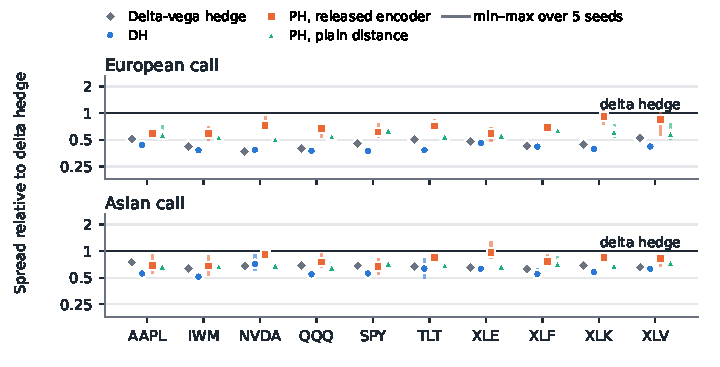
\includegraphics[width=\textwidth]{fig_tickers}
\caption{Spread of the hedging error by ticker, relative to the delta hedge (log scale; lower is better),
main setup, test period 2022--2024. Markers are seed means, bars the range over seeds.}
\label{fig:tickers}
\end{figure}

\paragraph{Hedging quality.} Table~\ref{tab:hedging} and Fig.~\ref{fig:tickers} compare the main setup
with rule-based hedges. Both learned methods have a narrower hedging-error spread than the delta hedge in
every ticker (296 of 300 fits). PH removes 88.5\% and 84.9\% of the risk, against 93.3\% and 88.7\% for DH;
its spread is wider than DH's in all ten tickers and its worst-5\% loss is larger (PH $-$ DH, in percent of
the initial price: std$(E)$ $+0.19$ $[0.16, 0.21]$ and $+0.09$ $[0.07, 0.11]$; CVaR$_5(E)$ $-0.43$
$[-0.51, -0.31]$ and $-0.16$ $[-0.25, -0.07]$; Holm-adjusted $p=0.006$ for all four). DH also beats a
delta--vega hedge in 9 of 10 tickers; PH does so in 0 (European) and 2 (Asian). This gap is new on real
data: in simulation PH's spread was within 3\% of DH's. The plain-distance layer hedges better than the
encoder (90.7\% and 87.2\% of the risk removed; a narrower spread in 9 and 8 of 10 tickers) but is
detectably behind DH on the original metric for the European call ($-0.00133$ $[-0.00187, -0.00080]$).

\paragraph{Training data.} Much of the gap is a data effect. On the validation data of the development
tickers, with a quarter of a ticker's history PH is no better than the delta hedge (spread 0.93 and 1.03
times the delta hedge's, against 0.42 and 0.65 for DH), and with all of it 0.51 and 0.64 (DH: 0.27 and
0.44). Training one model on all ten tickers narrows the gap most: on the test period, pooled PH removes
92.2\% and 88.8\% of the risk, pooled DH 94.0\% and 90.7\%.

% ------------------------------------------------------------------------------------------------
\section{Are the Explanations Real?}
\label{sec:explain}

\begin{table}[t]
\caption{Pre-declared explanation tests, test period 2022--2024, 100 fits per layer. Necessity: change of the decision in units of its standard deviation; sufficiency, self-consistency and
fallback: relative change of the spread or the output. \pass\ pass, \fail\ fail, by the mark recorded before
the run. For necessity the plain layer fails narrowly on the European call at the level of the whole hedge
(rank correlation 0.46 against a mark of 0.5). An untrained encoder with the same prototypes scores 65\% /
75\% on similarity.}
\label{tab:audit}
\centering
\scriptsize
\setlength{\tabcolsep}{3pt}
\begin{tabular}{@{}>{\raggedright\arraybackslash}p{1.6cm}>{\raggedright\arraybackslash}p{3.45cm}>{\raggedright\arraybackslash}p{0.8cm}cccc@{}}
\toprule
 & & & \multicolumn{2}{c}{Released encoder} & \multicolumn{2}{c}{Plain distance} \\
\cmidrule(lr){4-5}\cmidrule(l){6-7}
Test & Measure & Pass mark & European & Asian & European & Asian \\
\midrule
\multicolumn{7}{@{}l}{\emph{Influence}} \\
Stability & Heaviest prototype unchanged under 0.1 sd noise & $\ge$90\% & 94\% \textsc{p} & 91\% \textsc{p} & 92\% \textsc{p} & 94\% \textsc{p} \\
Local removal & Output change, 3 heaviest / 3 lightest removed (sd) & $\ge$3$\times$, $\le$0.05 & 0.63/0.00 \textsc{p} & 0.76/0.00 \textsc{p} & 0.35/0.01 \textsc{p} & 0.75/0.01 \textsc{p} \\
Deletion & Corr.\ of use with std$(E)$ rise on deletion & $\ge$0.5 & 0.69 \textsc{p} & 0.73 \textsc{p} & 0.46 \textsc{f} & 0.52 \textsc{p} \\
\midrule
\multicolumn{7}{@{}l}{\emph{Visible similarity}} \\
Nearest$^{\ddagger}$ & Heaviest is nearest of 10 (chance 10\%) & $\ge$50\% & 19\% \textsc{f} & 37\% \textsc{f} & 73\% \textsc{p} & 78\% \textsc{p} \\
\midrule
\multicolumn{7}{@{}l}{\emph{Crisis correspondence}} \\
Represent. & Prototypes in stress windows (9.4\% of days) & $\ge$14\% & 20\% \textsc{p} & 24\% \textsc{p} & 22\% \textsc{p} & 23\% \textsc{p} \\
Recall & Their weight, calm $\to$ stressed test days & rise & 17$\to$20\% \textsc{p} & 20$\to$26\% \textsc{p} & 13$\to$26\% \textsc{p} & 15$\to$28\% \textsc{p} \\
\midrule
\multicolumn{7}{@{}l}{\emph{Reading and use}} \\
Sufficiency$^{\ddagger}$ & std$(E)$ change, top 3 prototypes only & $\le$5\% & 7\% \textsc{f} & 15\% \textsc{f} & 63\% \textsc{f} & 35\% \textsc{f} \\
Self-consist. & Output at own state vs attached output (sd) & $\le$10\% & 14\% \textsc{f} & 23\% \textsc{f} & 18\% \textsc{f} & 28\% \textsc{f} \\
Fallback & std$(E)$ change, delta hedge far from bank & $<$0 & +15\% \textsc{f} & +12\% \textsc{f} & +23\% \textsc{f} & +11\% \textsc{f} \\
\bottomrule
\end{tabular}

\end{table}

\paragraph{Tests.} A decision's explanation consists of its prototype weights, the prototypes themselves
(dated real states) and their attached outputs. We fixed the tests and pass marks of Table~\ref{tab:audit}
before running them and applied them to all 100 main-setup fits of each layer on the test period.
Stability uses noise of 0.1 standard deviations on the market features, less than their median daily move
(0.14 to 0.20). Necessity also deletes each prototype from the model, which should hurt the hedge in
proportion to the prototype's use. The stress windows are six periods of 2008--2018 fixed from the public
record (the 2008--09 crisis, 2010, 2011, 2015 and two in 2018); stressed test days are the top 10\% by
implied volatility. Fallback acts when the state is farther from every prototype than 95\% of training
states.

\paragraph{Faithfulness.} Both layers give stable explanations, and the prototypes they name are the ones
that matter: removing the three heaviest changes the decision by 0.35 to 0.76 standard deviations, removing
the three lightest by at most 0.01. Deleting a prototype from the model hurts the hedge in proportion to its
use, except narrowly for the plain layer on the European call. The layers part on similarity. With the plain
distance the heaviest prototype is the nearest state in 73\% and 78\% of decisions; with the released encoder
in only 19\% and 37\%, against 10\% by chance. An untrained encoder with the same prototypes scores 65\% and
75\%, so it is training that moves the encoder's notion of similarity away from the features a reader can
see, the gap between latent and input similarity reported for image models \cite{hoffmann2021looks}. For the
plain layer the explanation is a weighted distance on named features, with most weight on the listed call's
log-moneyness (41\% and 32\%), followed by the positions held. Two readings of an explanation are only
approximate for both layers: hedging with the three heaviest prototypes alone changes the spread by 7\% to
63\%, and at a prototype's own state the model's output differs from the attached action by 14\% to 28\% of
the output scale.

\paragraph{Crises.} Prototypes are disproportionately crisis days: 20\% to 24\% of them come from the
stress windows, which hold 9.4\% of training days. On stressed test days the weight on them rises, clearly
for the plain layer (from 13\% to 26\% and from 15\% to 28\%) and modestly for the encoder (from 17\% to
20\% and from 20\% to 26\%); defining stress by named market events of 2022--2024 instead gives the same
result. A third test failed for both layers: the largest trades are not more often explained by crisis
prototypes. Since 94\% to 100\% of the largest trades open an episode, that test did not isolate defensive
trades.

\begin{figure}[t]
\centering
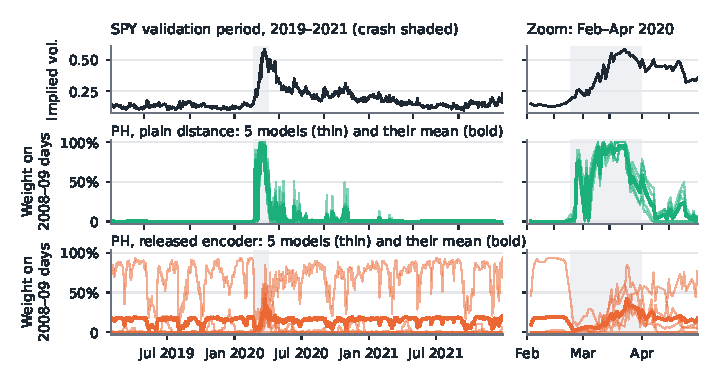
\includegraphics[width=\textwidth]{fig_covid}
\caption{SPY, European call, through the validation years, which no model trained on. Top: median implied
volatility of the listed calls. Bottom: share of the decision weight on prototypes dated in the 2008--09
financial crisis, daily average. One encoder model weights those prototypes heavily throughout (68\% in
2019); the encoder mean includes it.}
\label{fig:covid}
\end{figure}

\paragraph{A case: March 2020.} Figure~\ref{fig:covid} follows the SPY models through the validation
years. Their stopping epochs were chosen on these years, and we chose this case after the tests, reporting
all ten models. In 17 of SPY's 20 models one prototype is 29 September 2008, the day the US House of
Representatives rejected the bank bailout and the S\&P~500 fell 8.8\%. In that state SPY stood 10\% below
the start of its hedge and implied volatility was 48\%; the plain layer attaches to it the action ``keep
roughly the delta hedge in shares and add about a third of a listed call''. In calm 2019 the five
plain-distance models put essentially no weight (under 0.2\%) on 2008--09 crisis days. During the COVID crash
(24 February to 31 March 2020) they put 49\% to 71\% of their weight on them: the three models that keep
29 September 2008 chose it as their heaviest prototype, and the other two chose the first week of March
2009, just before that crisis's market bottom. On the worst days they held between 0.37 and 0.55 listed calls
on top of a small share position, close to the 2008 day's attached action, where a delta hedge would hold
0.09 shares and no options. Over the 20 hedges open on 16 March 2020, their average absolute hedging error
was 1.5\% of the initial price, against 2.7\% for the delta hedge, 3.6\% unhedged, 1.1\% for the encoder and
0.5\% for DH. The encoder made no such link: its average weight on 2008--09 days stayed near 15\% throughout.

\paragraph{A warning signal?} The distance from the current market state to the nearest prototype rises
with the size of the hedging error (rank correlation 0.14 to 0.25), but it mostly tracks implied volatility
(monthly correlation 0.93) and flags DH's difficult episodes as well. Falling back to the delta hedge far
from every prototype made hedging worse (Table~\ref{tab:audit}), and no better than falling back at random.

% ------------------------------------------------------------------------------------------------
\section{Limitations}

The liabilities are synthetic and the costs stylised; we study ten US underlyings and one maturity range.
About a hundred independent training months per underlying limit what any learned hedge can extract. The
test period was examined in an earlier version of this study, so the evaluation is a single pre-declared
look at a period that was not new to us. The explanation tests are functional rather than a user study, and
exploratory; two of their pass marks were set with the corresponding numbers known. The March 2020 case lies
in the validation period and was selected after the tests. Two of 100 encoder fits and 13 of 100
plain-distance fits reached the epoch limit.

% ------------------------------------------------------------------------------------------------
\section{Conclusion}

ProtoHedge's central claim survives the move to real option markets on its own terms: on the original
metric it is never detectably behind Deep Hedging, once both methods are set up to hedge. Its explanations
can be checked against market history and largely hold up: they are stable, they name the past states that
drive each decision, and in stressed markets they reach for past crises, clearly so with the plain-distance
layer, as the original paper anticipated. The price is a wider hedging error than Deep Hedging's, and with the released encoder the named
states are often not the most similar ones. For explanations that a reader can verify we recommend the
plain-distance layer; for the narrowest hedge, Deep Hedging remains ahead.

\paragraph{Data and code.} OptionMetrics and CRSP data are licensed through WRDS and cannot be
redistributed. Code, configurations and the pre-declared protocols are available from the authors on
request.

\bibliographystyle{splncs04}
\bibliography{references}

\end{document}
